\documentclass[1p]{elsarticle_modified}
%\bibliographystyle{elsarticle-num}

%\usepackage[colorlinks]{hyperref}
%\usepackage{abbrmath_seonhwa} %\Abb, \Ascr, \Acal ,\Abf, \Afrak
\usepackage{amsfonts}
\usepackage{amssymb}
\usepackage{amsmath}
\usepackage{amsthm}
\usepackage{scalefnt}
\usepackage{amsbsy}
\usepackage{kotex}
\usepackage{caption}
\usepackage{subfig}
\usepackage{color}
\usepackage{graphicx}
\usepackage{xcolor} %% white, black, red, green, blue, cyan, magenta, yellow
\usepackage{float}
\usepackage{setspace}
\usepackage{hyperref}

\usepackage{tikz}
\usetikzlibrary{arrows}

\usepackage{multirow}
\usepackage{array} % fixed length table
\usepackage{hhline}

%%%%%%%%%%%%%%%%%%%%%
\makeatletter
\renewcommand*\env@matrix[1][\arraystretch]{%
	\edef\arraystretch{#1}%
	\hskip -\arraycolsep
	\let\@ifnextchar\new@ifnextchar
	\array{*\c@MaxMatrixCols c}}
\makeatother %https://tex.stackexchange.com/questions/14071/how-can-i-increase-the-line-spacing-in-a-matrix
%%%%%%%%%%%%%%%

\usepackage[normalem]{ulem}

\newcommand{\msout}[1]{\ifmmode\text{\sout{\ensuremath{#1}}}\else\sout{#1}\fi}
%SOURCE: \msout is \stkout macro in https://tex.stackexchange.com/questions/20609/strikeout-in-math-mode

\newcommand{\cancel}[1]{
	\ifmmode
	{\color{red}\msout{#1}}
	\else
	{\color{red}\sout{#1}}
	\fi
}

\newcommand{\add}[1]{
	{\color{blue}\uwave{#1}}
}

\newcommand{\replace}[2]{
	\ifmmode
	{\color{red}\msout{#1}}{\color{blue}\uwave{#2}}
	\else
	{\color{red}\sout{#1}}{\color{blue}\uwave{#2}}
	\fi
}

\newcommand{\Sol}{\mathcal{S}} %segment
\newcommand{\D}{D} %diagram
\newcommand{\A}{\mathcal{A}} %arc


%%%%%%%%%%%%%%%%%%%%%%%%%%%%%5 test

\def\sl{\operatorname{\textup{SL}}(2,\Cbb)}
\def\psl{\operatorname{\textup{PSL}}(2,\Cbb)}
\def\quan{\mkern 1mu \triangleright \mkern 1mu}

\theoremstyle{definition}
\newtheorem{thm}{Theorem}[section]
\newtheorem{prop}[thm]{Proposition}
\newtheorem{lem}[thm]{Lemma}
\newtheorem{ques}[thm]{Question}
\newtheorem{cor}[thm]{Corollary}
\newtheorem{defn}[thm]{Definition}
\newtheorem{exam}[thm]{Example}
\newtheorem{rmk}[thm]{Remark}
\newtheorem{alg}[thm]{Algorithm}

\newcommand{\I}{\sqrt{-1}}
\begin{document}

%\begin{frontmatter}
%
%\title{Boundary parabolic representations of knots up to 8 crossings}
%
%%% Group authors per affiliation:
%\author{Yunhi Cho} 
%\address{Department of Mathematics, University of Seoul, Seoul, Korea}
%\ead{yhcho@uos.ac.kr}
%
%
%\author{Seonhwa Kim} %\fnref{s_kim}}
%\address{Center for Geometry and Physics, Institute for Basic Science, Pohang, 37673, Korea}
%\ead{ryeona17@ibs.re.kr}
%
%\author{Hyuk Kim}
%\address{Department of Mathematical Sciences, Seoul National University, Seoul 08826, Korea}
%\ead{hyukkim@snu.ac.kr}
%
%\author{Seokbeom Yoon}
%\address{Department of Mathematical Sciences, Seoul National University, Seoul, 08826,  Korea}
%\ead{sbyoon15@snu.ac.kr}
%
%\begin{abstract}
%We find all boundary parabolic representation of knots up to 8 crossings.
%
%\end{abstract}
%\begin{keyword}
%    \MSC[2010] 57M25 
%\end{keyword}
%
%\end{frontmatter}

%\linenumbers
%\tableofcontents
%
\newcommand\colored[1]{\textcolor{white}{\rule[-0.35ex]{0.8em}{1.4ex}}\kern-0.8em\color{red} #1}%
%\newcommand\colored[1]{\textcolor{white}{ #1}\kern-2.17ex	\textcolor{white}{ #1}\kern-1.81ex	\textcolor{white}{ #1}\kern-2.15ex\color{red}#1	}

{\Large $\underline{11a_{35}~(K11a_{35})}$}

\setlength{\tabcolsep}{10pt}
\renewcommand{\arraystretch}{1.6}
\vspace{1cm}\begin{tabular}{m{100pt}>{\centering\arraybackslash}m{274pt}}
\multirow{5}{120pt}{
	\centering
	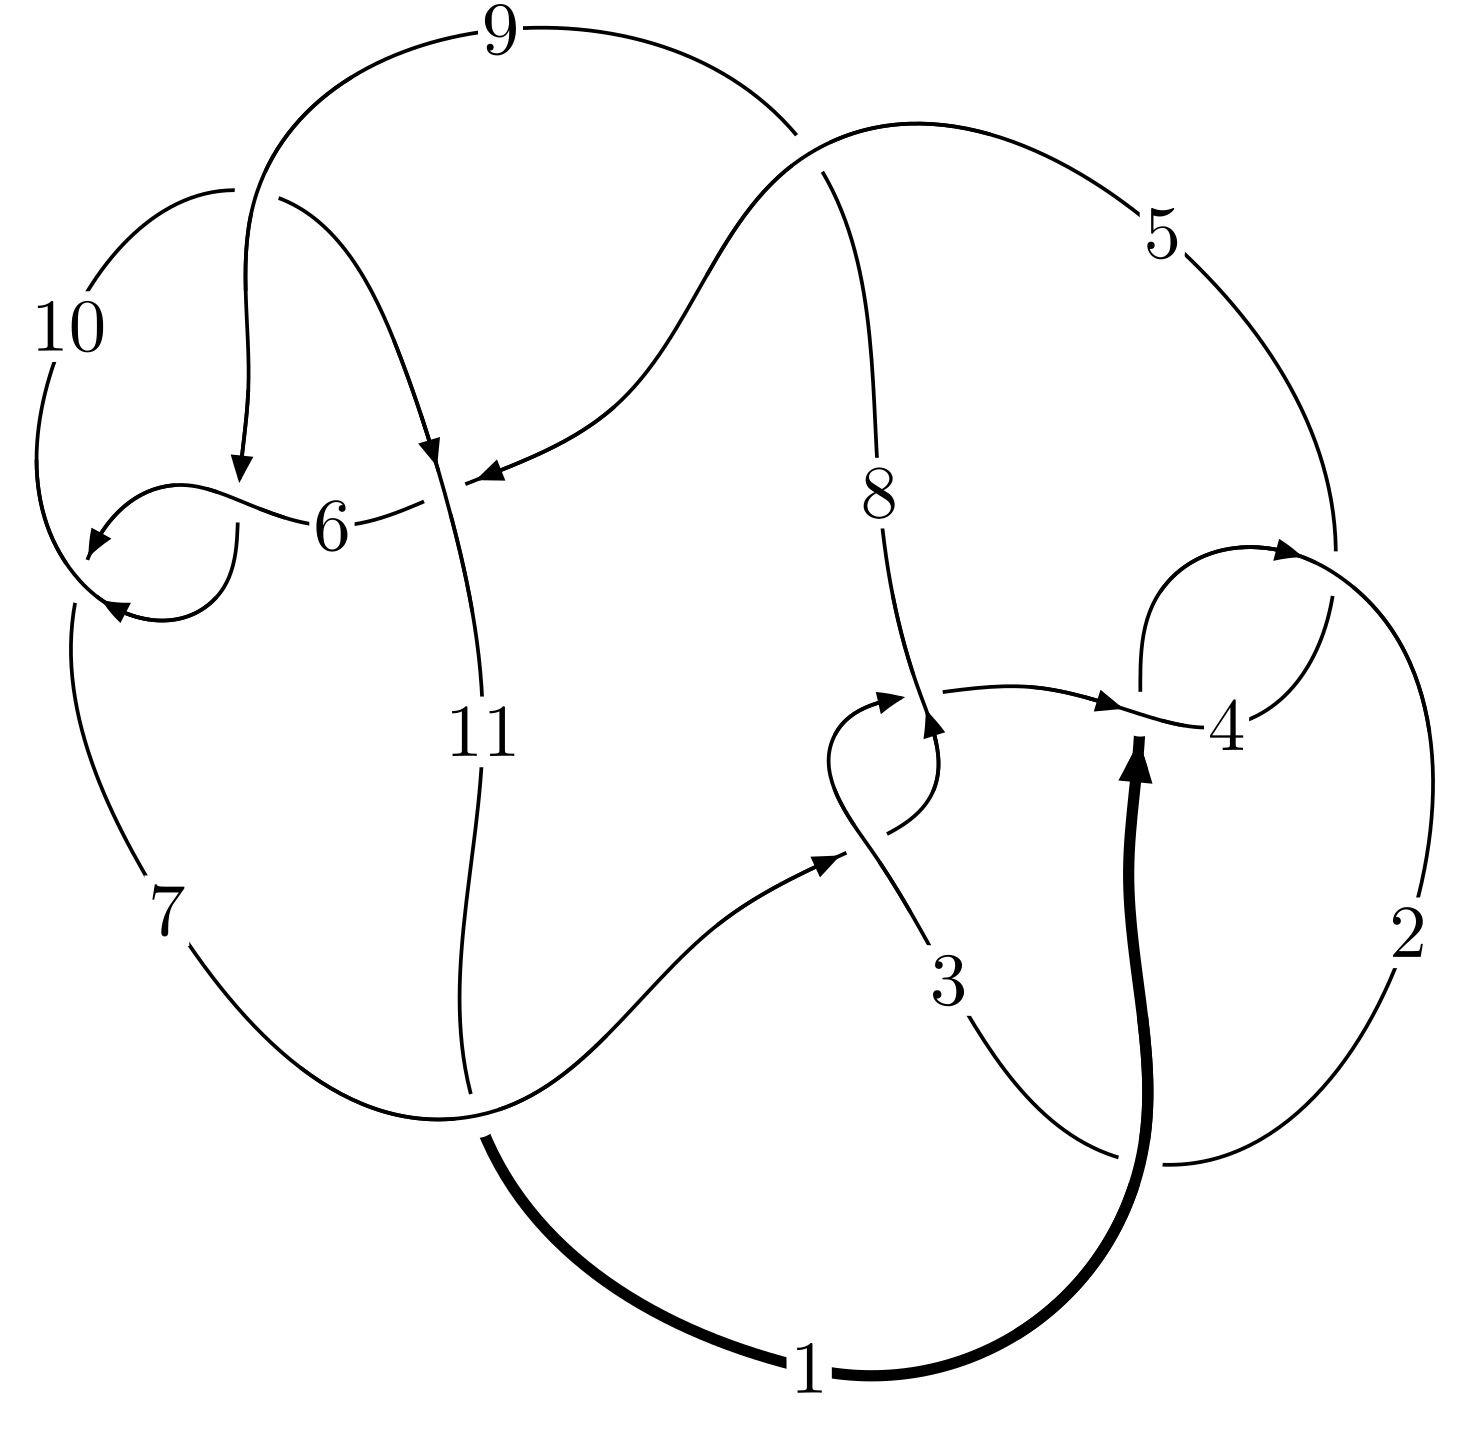
\includegraphics[width=112pt]{../../../GIT/diagram.site/Diagrams/png/284_11a_35.png}\\
\ \ \ A knot diagram\footnotemark}&
\allowdisplaybreaks
\textbf{Linearized knot diagam} \\
\cline{2-2}
 &
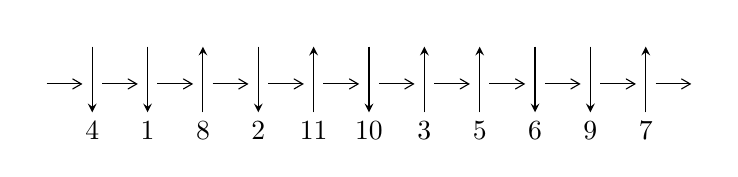
\begin{tikzpicture}[x=20pt, y=17pt]
	% nodes
	\node (C0) at (0, 0) {};
	\node (C1) at (1, 0) {};
	\node (C1U) at (1, +1) {};
	\node (C1D) at (1, -1) {4};

	\node (C2) at (2, 0) {};
	\node (C2U) at (2, +1) {};
	\node (C2D) at (2, -1) {1};

	\node (C3) at (3, 0) {};
	\node (C3U) at (3, +1) {};
	\node (C3D) at (3, -1) {8};

	\node (C4) at (4, 0) {};
	\node (C4U) at (4, +1) {};
	\node (C4D) at (4, -1) {2};

	\node (C5) at (5, 0) {};
	\node (C5U) at (5, +1) {};
	\node (C5D) at (5, -1) {11};

	\node (C6) at (6, 0) {};
	\node (C6U) at (6, +1) {};
	\node (C6D) at (6, -1) {10};

	\node (C7) at (7, 0) {};
	\node (C7U) at (7, +1) {};
	\node (C7D) at (7, -1) {3};

	\node (C8) at (8, 0) {};
	\node (C8U) at (8, +1) {};
	\node (C8D) at (8, -1) {5};

	\node (C9) at (9, 0) {};
	\node (C9U) at (9, +1) {};
	\node (C9D) at (9, -1) {6};

	\node (C10) at (10, 0) {};
	\node (C10U) at (10, +1) {};
	\node (C10D) at (10, -1) {9};

	\node (C11) at (11, 0) {};
	\node (C11U) at (11, +1) {};
	\node (C11D) at (11, -1) {7};
	\node (C12) at (12, 0) {};

	% arrows
	\draw[->,>={angle 60}]
	(C0) edge (C1) (C1) edge (C2) (C2) edge (C3) (C3) edge (C4) (C4) edge (C5) (C5) edge (C6) (C6) edge (C7) (C7) edge (C8) (C8) edge (C9) (C9) edge (C10) (C10) edge (C11) (C11) edge (C12) ;	\draw[->,>=stealth]
	(C1U) edge (C1D) (C2U) edge (C2D) (C3D) edge (C3U) (C4U) edge (C4D) (C5D) edge (C5U) (C6U) edge (C6D) (C7D) edge (C7U) (C8D) edge (C8U) (C9U) edge (C9D) (C10U) edge (C10D) (C11D) edge (C11U) ;
	\end{tikzpicture} \\
\hhline{~~} \\& 
\textbf{Solving Sequence} \\ \cline{2-2} 
 &
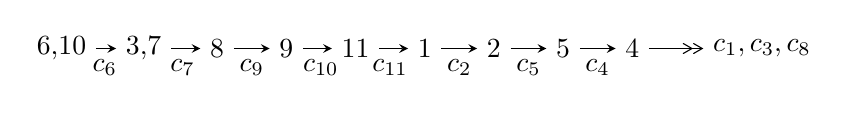
\begin{tikzpicture}[x=25pt, y=7pt]
	% node
	\node (A0) at (-1/8, 0) {6,10};
	\node (A1) at (17/16, 0) {3,7};
	\node (A2) at (17/8, 0) {8};
	\node (A3) at (25/8, 0) {9};
	\node (A4) at (33/8, 0) {11};
	\node (A5) at (41/8, 0) {1};
	\node (A6) at (49/8, 0) {2};
	\node (A7) at (57/8, 0) {5};
	\node (A8) at (65/8, 0) {4};
	\node (C1) at (1/2, -1) {$c_{6}$};
	\node (C2) at (13/8, -1) {$c_{7}$};
	\node (C3) at (21/8, -1) {$c_{9}$};
	\node (C4) at (29/8, -1) {$c_{10}$};
	\node (C5) at (37/8, -1) {$c_{11}$};
	\node (C6) at (45/8, -1) {$c_{2}$};
	\node (C7) at (53/8, -1) {$c_{5}$};
	\node (C8) at (61/8, -1) {$c_{4}$};
	\node (A9) at (10, 0) {$c_{1},c_{3},c_{8}$};

	% edge
	\draw[->,>=stealth]	
	(A0) edge (A1) (A1) edge (A2) (A2) edge (A3) (A3) edge (A4) (A4) edge (A5) (A5) edge (A6) (A6) edge (A7) (A7) edge (A8) ;
	\draw[->>,>={angle 60}]	
	(A8) edge (A9);
\end{tikzpicture} \\ 

\end{tabular} \\

\footnotetext{
The image of knot diagram is generated by the software ``\textbf{Draw programme}" developed by Andrew Bartholomew(\url{http://www.layer8.co.uk/maths/draw/index.htm\#Running-draw}), where we modified some parts for our purpose(\url{https://github.com/CATsTAILs/LinksPainter}).
}\phantom \\ \newline 
\centering \textbf{Ideals for irreducible components\footnotemark of $X_{\text{par}}$} 
 
\begin{align*}
I^u_{1}&=\langle 
2 u^{65}- u^{64}+\cdots- u^2+b,\;u^{64}+u^{63}+\cdots+a+1,\;u^{66}-2 u^{65}+\cdots- u+1\rangle \\
I^u_{2}&=\langle 
- u^3+b+u+1,\;- u^4- u^3+u^2+a+u,\;u^6+u^5- u^4-2 u^3+u+1\rangle \\
\\
\end{align*}
\raggedright * 2 irreducible components of $\dim_{\mathbb{C}}=0$, with total 72 representations.\\
\footnotetext{All coefficients of polynomials are rational numbers. But the coefficients are sometimes approximated in decimal forms when there is not enough margin.}
\newpage
\renewcommand{\arraystretch}{1}
\centering \section*{I. $I^u_{1}= \langle 2 u^{65}- u^{64}+\cdots- u^2+b,\;u^{64}+u^{63}+\cdots+a+1,\;u^{66}-2 u^{65}+\cdots- u+1 \rangle$}
\flushleft \textbf{(i) Arc colorings}\\
\begin{tabular}{m{7pt} m{180pt} m{7pt} m{180pt} }
\flushright $a_{6}=$&$\begin{pmatrix}1\\0\end{pmatrix}$ \\
\flushright $a_{10}=$&$\begin{pmatrix}0\\u\end{pmatrix}$ \\
\flushright $a_{3}=$&$\begin{pmatrix}- u^{64}- u^{63}+\cdots- u^2-1\\-2 u^{65}+u^{64}+\cdots-8 u^4+u^2\end{pmatrix}$ \\
\flushright $a_{7}=$&$\begin{pmatrix}1\\u^2\end{pmatrix}$ \\
\flushright $a_{8}=$&$\begin{pmatrix}- u^{11}+2 u^9-2 u^7+u^3\\- u^{11}+3 u^9-4 u^7+3 u^5- u^3+u\end{pmatrix}$ \\
\flushright $a_{9}=$&$\begin{pmatrix}u\\u\end{pmatrix}$ \\
\flushright $a_{11}=$&$\begin{pmatrix}- u^3\\- u^3+u\end{pmatrix}$ \\
\flushright $a_{1}=$&$\begin{pmatrix}u^5-2 u^3+u\\u^7- u^5+u\end{pmatrix}$ \\
\flushright $a_{2}=$&$\begin{pmatrix}- u^{63}+u^{62}+\cdots- u-1\\- u^{65}+u^{64}+\cdots+u^3+u^2\end{pmatrix}$ \\
\flushright $a_{5}=$&$\begin{pmatrix}u^6- u^4+1\\u^6-2 u^4+u^2\end{pmatrix}$ \\
\flushright $a_{4}=$&$\begin{pmatrix}u^{64}- u^{63}+\cdots- u^2- u\\u^{64}- u^{63}+\cdots+u^2+u\end{pmatrix}$\\ \flushright $a_{4}=$&$\begin{pmatrix}u^{64}- u^{63}+\cdots- u^2- u\\u^{64}- u^{63}+\cdots+u^2+u\end{pmatrix}$\\&\end{tabular}
\flushleft \textbf{(ii) Obstruction class $= -1$}\\~\\
\flushleft \textbf{(iii) Cusp Shapes $= 4 u^{65}-6 u^{64}+\cdots-4 u-6$}\\~\\
\newpage\renewcommand{\arraystretch}{1}
\flushleft \textbf{(iv) u-Polynomials at the component}\newline \\
\begin{tabular}{m{50pt}|m{274pt}}
Crossings & \hspace{64pt}u-Polynomials at each crossing \\
\hline $$\begin{aligned}c_{1},c_{4}\end{aligned}$$&$\begin{aligned}
&u^{66}-7 u^{65}+\cdots-8 u+1
\end{aligned}$\\
\hline $$\begin{aligned}c_{2}\end{aligned}$$&$\begin{aligned}
&u^{66}+29 u^{65}+\cdots+8 u+1
\end{aligned}$\\
\hline $$\begin{aligned}c_{3},c_{7}\end{aligned}$$&$\begin{aligned}
&u^{66}+u^{65}+\cdots+192 u+64
\end{aligned}$\\
\hline $$\begin{aligned}c_{5}\end{aligned}$$&$\begin{aligned}
&u^{66}+6 u^{65}+\cdots+5 u+1
\end{aligned}$\\
\hline $$\begin{aligned}c_{6},c_{9}\end{aligned}$$&$\begin{aligned}
&u^{66}+2 u^{65}+\cdots+u+1
\end{aligned}$\\
\hline $$\begin{aligned}c_{8},c_{11}\end{aligned}$$&$\begin{aligned}
&u^{66}-2 u^{65}+\cdots-49 u+49
\end{aligned}$\\
\hline $$\begin{aligned}c_{10}\end{aligned}$$&$\begin{aligned}
&u^{66}+30 u^{65}+\cdots- u+1
\end{aligned}$\\
\hline
\end{tabular}\\~\\
\newpage\renewcommand{\arraystretch}{1}
\flushleft \textbf{(v) Riley Polynomials at the component}\newline \\
\begin{tabular}{m{50pt}|m{274pt}}
Crossings & \hspace{64pt}Riley Polynomials at each crossing \\
\hline $$\begin{aligned}c_{1},c_{4}\end{aligned}$$&$\begin{aligned}
&y^{66}-29 y^{65}+\cdots-8 y+1
\end{aligned}$\\
\hline $$\begin{aligned}c_{2}\end{aligned}$$&$\begin{aligned}
&y^{66}+23 y^{65}+\cdots+40 y+1
\end{aligned}$\\
\hline $$\begin{aligned}c_{3},c_{7}\end{aligned}$$&$\begin{aligned}
&y^{66}-39 y^{65}+\cdots-81920 y+4096
\end{aligned}$\\
\hline $$\begin{aligned}c_{5}\end{aligned}$$&$\begin{aligned}
&y^{66}+2 y^{65}+\cdots+57 y+1
\end{aligned}$\\
\hline $$\begin{aligned}c_{6},c_{9}\end{aligned}$$&$\begin{aligned}
&y^{66}-30 y^{65}+\cdots+y+1
\end{aligned}$\\
\hline $$\begin{aligned}c_{8},c_{11}\end{aligned}$$&$\begin{aligned}
&y^{66}-54 y^{65}+\cdots+34349 y+2401
\end{aligned}$\\
\hline $$\begin{aligned}c_{10}\end{aligned}$$&$\begin{aligned}
&y^{66}+14 y^{65}+\cdots-15 y+1
\end{aligned}$\\
\hline
\end{tabular}\\~\\
\newpage\flushleft \textbf{(vi) Complex Volumes and Cusp Shapes}
$$\begin{array}{c|c|c}  
\text{Solutions to }I^u_{1}& \I (\text{vol} + \sqrt{-1}CS) & \text{Cusp shape}\\
 \hline 
\begin{aligned}
u &= -0.838382 + 0.570498 I \\
a &= -1.59137 + 0.96841 I \\
b &= -0.89229 + 1.65118 I\end{aligned}
 & \phantom{-}2.86632 + 4.91582 I & \phantom{-}3.89105 - 6.54024 I \\ \hline\begin{aligned}
u &= -0.838382 - 0.570498 I \\
a &= -1.59137 - 0.96841 I \\
b &= -0.89229 - 1.65118 I\end{aligned}
 & \phantom{-}2.86632 - 4.91582 I & \phantom{-}3.89105 + 6.54024 I \\ \hline\begin{aligned}
u &= \phantom{-}1.033280 + 0.092662 I \\
a &= \phantom{-}0.186149 - 0.978915 I \\
b &= \phantom{-}0.1030790 - 0.0082510 I\end{aligned}
 & -1.69775 + 2.04297 I & -4.04234 - 3.06094 I \\ \hline\begin{aligned}
u &= \phantom{-}1.033280 - 0.092662 I \\
a &= \phantom{-}0.186149 + 0.978915 I \\
b &= \phantom{-}0.1030790 + 0.0082510 I\end{aligned}
 & -1.69775 - 2.04297 I & -4.04234 + 3.06094 I \\ \hline\begin{aligned}
u &= \phantom{-}0.982840 + 0.372620 I \\
a &= \phantom{-}0.374917 + 0.408622 I \\
b &= -0.326106 + 0.086039 I\end{aligned}
 & -1.69198 - 1.38184 I & \phantom{-0.000000 } 0 \\ \hline\begin{aligned}
u &= \phantom{-}0.982840 - 0.372620 I \\
a &= \phantom{-}0.374917 - 0.408622 I \\
b &= -0.326106 - 0.086039 I\end{aligned}
 & -1.69198 + 1.38184 I & \phantom{-0.000000 } 0 \\ \hline\begin{aligned}
u &= -0.933351 + 0.146746 I \\
a &= -1.76404 - 0.58789 I \\
b &= -2.40628 + 0.14225 I\end{aligned}
 & -2.87483 + 0.09947 I & -1.36414 + 2.00887 I \\ \hline\begin{aligned}
u &= -0.933351 - 0.146746 I \\
a &= -1.76404 + 0.58789 I \\
b &= -2.40628 - 0.14225 I\end{aligned}
 & -2.87483 - 0.09947 I & -1.36414 - 2.00887 I \\ \hline\begin{aligned}
u &= -0.742441 + 0.572901 I \\
a &= \phantom{-}1.41865 - 0.89922 I \\
b &= \phantom{-}0.73516 - 1.51912 I\end{aligned}
 & \phantom{-}3.13736 - 0.33428 I & \phantom{-}4.85916 - 0.25871 I \\ \hline\begin{aligned}
u &= -0.742441 - 0.572901 I \\
a &= \phantom{-}1.41865 + 0.89922 I \\
b &= \phantom{-}0.73516 + 1.51912 I\end{aligned}
 & \phantom{-}3.13736 + 0.33428 I & \phantom{-}4.85916 + 0.25871 I\\
 \hline 
 \end{array}$$\newpage$$\begin{array}{c|c|c}  
\text{Solutions to }I^u_{1}& \I (\text{vol} + \sqrt{-1}CS) & \text{Cusp shape}\\
 \hline 
\begin{aligned}
u &= \phantom{-}0.548886 + 0.758609 I \\
a &= \phantom{-}2.42346 + 0.19818 I \\
b &= \phantom{-}0.51274 + 1.38998 I\end{aligned}
 & \phantom{-}7.33465 - 7.05782 I & \phantom{-}4.34818 + 5.54118 I \\ \hline\begin{aligned}
u &= \phantom{-}0.548886 - 0.758609 I \\
a &= \phantom{-}2.42346 - 0.19818 I \\
b &= \phantom{-}0.51274 - 1.38998 I\end{aligned}
 & \phantom{-}7.33465 + 7.05782 I & \phantom{-}4.34818 - 5.54118 I \\ \hline\begin{aligned}
u &= \phantom{-}0.521388 + 0.768999 I \\
a &= -2.49233 - 0.13326 I \\
b &= -0.48790 - 1.63707 I\end{aligned}
 & \phantom{-}9.01786 - 1.00374 I & \phantom{-}6.50365 + 0.74875 I \\ \hline\begin{aligned}
u &= \phantom{-}0.521388 - 0.768999 I \\
a &= -2.49233 + 0.13326 I \\
b &= -0.48790 + 1.63707 I\end{aligned}
 & \phantom{-}9.01786 + 1.00374 I & \phantom{-}6.50365 - 0.74875 I \\ \hline\begin{aligned}
u &= \phantom{-}0.449304 + 0.792107 I \\
a &= -2.35386 + 0.17418 I \\
b &= -0.48979 - 2.15203 I\end{aligned}
 & \phantom{-}8.61616 + 4.06846 I & \phantom{-}6.02832 - 1.29392 I \\ \hline\begin{aligned}
u &= \phantom{-}0.449304 - 0.792107 I \\
a &= -2.35386 - 0.17418 I \\
b &= -0.48979 + 2.15203 I\end{aligned}
 & \phantom{-}8.61616 - 4.06846 I & \phantom{-}6.02832 + 1.29392 I \\ \hline\begin{aligned}
u &= \phantom{-}0.426139 + 0.798466 I \\
a &= \phantom{-}2.20027 - 0.25612 I \\
b &= \phantom{-}0.48809 + 2.24847 I\end{aligned}
 & \phantom{-}6.65145 + 10.08610 I & \phantom{-}3.42420 - 5.72376 I \\ \hline\begin{aligned}
u &= \phantom{-}0.426139 - 0.798466 I \\
a &= \phantom{-}2.20027 + 0.25612 I \\
b &= \phantom{-}0.48809 - 2.24847 I\end{aligned}
 & \phantom{-}6.65145 - 10.08610 I & \phantom{-}3.42420 + 5.72376 I \\ \hline\begin{aligned}
u &= -1.101690 + 0.070988 I \\
a &= \phantom{-}0.241428 + 0.643348 I \\
b &= \phantom{-}1.68689 + 0.38049 I\end{aligned}
 & \phantom{-}3.30286 - 2.13568 I & \phantom{-0.000000 } 0 \\ \hline\begin{aligned}
u &= -1.101690 - 0.070988 I \\
a &= \phantom{-}0.241428 - 0.643348 I \\
b &= \phantom{-}1.68689 - 0.38049 I\end{aligned}
 & \phantom{-}3.30286 + 2.13568 I & \phantom{-0.000000 } 0\\
 \hline 
 \end{array}$$\newpage$$\begin{array}{c|c|c}  
\text{Solutions to }I^u_{1}& \I (\text{vol} + \sqrt{-1}CS) & \text{Cusp shape}\\
 \hline 
\begin{aligned}
u &= -0.494791 + 0.742001 I \\
a &= \phantom{-}0.141507 - 0.914994 I \\
b &= -0.553428 - 0.923968 I\end{aligned}
 & \phantom{-}3.55117 + 1.02644 I & \phantom{-}3.26543 - 2.61936 I \\ \hline\begin{aligned}
u &= -0.494791 - 0.742001 I \\
a &= \phantom{-}0.141507 + 0.914994 I \\
b &= -0.553428 + 0.923968 I\end{aligned}
 & \phantom{-}3.55117 - 1.02644 I & \phantom{-}3.26543 + 2.61936 I \\ \hline\begin{aligned}
u &= -0.450858 + 0.762088 I \\
a &= \phantom{-}0.129006 + 0.877411 I \\
b &= \phantom{-}0.821517 + 0.695767 I\end{aligned}
 & \phantom{-}3.30665 - 3.77744 I & \phantom{-}2.64079 + 3.14160 I \\ \hline\begin{aligned}
u &= -0.450858 - 0.762088 I \\
a &= \phantom{-}0.129006 - 0.877411 I \\
b &= \phantom{-}0.821517 - 0.695767 I\end{aligned}
 & \phantom{-}3.30665 + 3.77744 I & \phantom{-}2.64079 - 3.14160 I \\ \hline\begin{aligned}
u &= -1.044040 + 0.415972 I \\
a &= \phantom{-}1.15918 - 2.16322 I \\
b &= -0.17820 - 2.43166 I\end{aligned}
 & -4.43668 + 2.24930 I & \phantom{-0.000000 } 0 \\ \hline\begin{aligned}
u &= -1.044040 - 0.415972 I \\
a &= \phantom{-}1.15918 + 2.16322 I \\
b &= -0.17820 + 2.43166 I\end{aligned}
 & -4.43668 - 2.24930 I & \phantom{-0.000000 } 0 \\ \hline\begin{aligned}
u &= \phantom{-}1.089680 + 0.276870 I \\
a &= \phantom{-}0.758755 - 0.342040 I \\
b &= \phantom{-}0.185758 + 0.260377 I\end{aligned}
 & -2.52561 - 2.07395 I & \phantom{-0.000000 } 0 \\ \hline\begin{aligned}
u &= \phantom{-}1.089680 - 0.276870 I \\
a &= \phantom{-}0.758755 + 0.342040 I \\
b &= \phantom{-}0.185758 - 0.260377 I\end{aligned}
 & -2.52561 + 2.07395 I & \phantom{-0.000000 } 0 \\ \hline\begin{aligned}
u &= \phantom{-}0.810413 + 0.329181 I \\
a &= \phantom{-}0.369859 + 0.669286 I \\
b &= -0.177061 - 0.174366 I\end{aligned}
 & -1.21777 - 1.53610 I & -1.19079 + 4.33474 I \\ \hline\begin{aligned}
u &= \phantom{-}0.810413 - 0.329181 I \\
a &= \phantom{-}0.369859 - 0.669286 I \\
b &= -0.177061 + 0.174366 I\end{aligned}
 & -1.21777 + 1.53610 I & -1.19079 - 4.33474 I\\
 \hline 
 \end{array}$$\newpage$$\begin{array}{c|c|c}  
\text{Solutions to }I^u_{1}& \I (\text{vol} + \sqrt{-1}CS) & \text{Cusp shape}\\
 \hline 
\begin{aligned}
u &= \phantom{-}0.465311 + 0.740633 I \\
a &= \phantom{-}2.81892 - 0.14269 I \\
b &= \phantom{-}0.15580 + 2.05972 I\end{aligned}
 & \phantom{-}1.86956 + 1.30967 I & \phantom{-}3.95870 - 0.74968 I \\ \hline\begin{aligned}
u &= \phantom{-}0.465311 - 0.740633 I \\
a &= \phantom{-}2.81892 + 0.14269 I \\
b &= \phantom{-}0.15580 - 2.05972 I\end{aligned}
 & \phantom{-}1.86956 - 1.30967 I & \phantom{-}3.95870 + 0.74968 I \\ \hline\begin{aligned}
u &= -1.121160 + 0.108789 I \\
a &= -0.098711 - 1.028630 I \\
b &= -1.64518 - 0.65204 I\end{aligned}
 & \phantom{-}1.42265 - 7.90790 I & \phantom{-0.000000 } 0 \\ \hline\begin{aligned}
u &= -1.121160 - 0.108789 I \\
a &= -0.098711 + 1.028630 I \\
b &= -1.64518 + 0.65204 I\end{aligned}
 & \phantom{-}1.42265 + 7.90790 I & \phantom{-0.000000 } 0 \\ \hline\begin{aligned}
u &= \phantom{-}1.057400 + 0.449933 I \\
a &= -0.603625 - 0.892474 I \\
b &= \phantom{-}0.834057 - 0.646276 I\end{aligned}
 & -4.18666 - 4.48001 I & \phantom{-0.000000 } 0 \\ \hline\begin{aligned}
u &= \phantom{-}1.057400 - 0.449933 I \\
a &= -0.603625 + 0.892474 I \\
b &= \phantom{-}0.834057 + 0.646276 I\end{aligned}
 & -4.18666 + 4.48001 I & \phantom{-0.000000 } 0 \\ \hline\begin{aligned}
u &= \phantom{-}1.108820 + 0.356169 I \\
a &= -1.058710 - 0.172368 I \\
b &= -0.049081 - 0.608014 I\end{aligned}
 & -3.31662 + 1.71384 I & \phantom{-0.000000 } 0 \\ \hline\begin{aligned}
u &= \phantom{-}1.108820 - 0.356169 I \\
a &= -1.058710 + 0.172368 I \\
b &= -0.049081 + 0.608014 I\end{aligned}
 & -3.31662 - 1.71384 I & \phantom{-0.000000 } 0 \\ \hline\begin{aligned}
u &= -1.059680 + 0.504654 I \\
a &= -0.61218 + 1.30860 I \\
b &= \phantom{-}0.134064 + 1.396220 I\end{aligned}
 & -0.63612 + 4.98818 I & \phantom{-0.000000 } 0 \\ \hline\begin{aligned}
u &= -1.059680 - 0.504654 I \\
a &= -0.61218 - 1.30860 I \\
b &= \phantom{-}0.134064 - 1.396220 I\end{aligned}
 & -0.63612 - 4.98818 I & \phantom{-0.000000 } 0\\
 \hline 
 \end{array}$$\newpage$$\begin{array}{c|c|c}  
\text{Solutions to }I^u_{1}& \I (\text{vol} + \sqrt{-1}CS) & \text{Cusp shape}\\
 \hline 
\begin{aligned}
u &= \phantom{-}1.032540 + 0.629706 I \\
a &= -1.02242 - 1.17537 I \\
b &= -0.51019 - 2.65763 I\end{aligned}
 & \phantom{-}5.89418 + 1.80044 I & \phantom{-0.000000 } 0 \\ \hline\begin{aligned}
u &= \phantom{-}1.032540 - 0.629706 I \\
a &= -1.02242 + 1.17537 I \\
b &= -0.51019 + 2.65763 I\end{aligned}
 & \phantom{-}5.89418 - 1.80044 I & \phantom{-0.000000 } 0 \\ \hline\begin{aligned}
u &= -1.114920 + 0.476437 I \\
a &= \phantom{-}0.19529 - 1.93571 I \\
b &= -0.80083 - 1.66249 I\end{aligned}
 & -2.51518 + 9.28456 I & \phantom{-0.000000 } 0 \\ \hline\begin{aligned}
u &= -1.114920 - 0.476437 I \\
a &= \phantom{-}0.19529 + 1.93571 I \\
b &= -0.80083 + 1.66249 I\end{aligned}
 & -2.51518 - 9.28456 I & \phantom{-0.000000 } 0 \\ \hline\begin{aligned}
u &= -1.059930 + 0.604349 I \\
a &= -1.346760 - 0.025560 I \\
b &= -1.163210 + 0.605646 I\end{aligned}
 & \phantom{-}1.87224 + 4.09931 I & \phantom{-0.000000 } 0 \\ \hline\begin{aligned}
u &= -1.059930 - 0.604349 I \\
a &= -1.346760 + 0.025560 I \\
b &= -1.163210 - 0.605646 I\end{aligned}
 & \phantom{-}1.87224 - 4.09931 I & \phantom{-0.000000 } 0 \\ \hline\begin{aligned}
u &= -1.094230 + 0.542575 I \\
a &= \phantom{-}0.187399 + 1.008530 I \\
b &= \phantom{-}0.634544 + 0.749712 I\end{aligned}
 & -0.78414 + 5.20993 I & \phantom{-0.000000 } 0 \\ \hline\begin{aligned}
u &= -1.094230 - 0.542575 I \\
a &= \phantom{-}0.187399 - 1.008530 I \\
b &= \phantom{-}0.634544 - 0.749712 I\end{aligned}
 & -0.78414 - 5.20993 I & \phantom{-0.000000 } 0 \\ \hline\begin{aligned}
u &= \phantom{-}1.052280 + 0.627132 I \\
a &= \phantom{-}1.32954 + 1.37112 I \\
b &= \phantom{-}0.54238 + 3.01297 I\end{aligned}
 & \phantom{-}7.43584 - 4.27253 I & \phantom{-0.000000 } 0 \\ \hline\begin{aligned}
u &= \phantom{-}1.052280 - 0.627132 I \\
a &= \phantom{-}1.32954 - 1.37112 I \\
b &= \phantom{-}0.54238 - 3.01297 I\end{aligned}
 & \phantom{-}7.43584 + 4.27253 I & \phantom{-0.000000 } 0\\
 \hline 
 \end{array}$$\newpage$$\begin{array}{c|c|c}  
\text{Solutions to }I^u_{1}& \I (\text{vol} + \sqrt{-1}CS) & \text{Cusp shape}\\
 \hline 
\begin{aligned}
u &= \phantom{-}1.074260 + 0.597515 I \\
a &= -2.18165 - 1.45852 I \\
b &= -0.87622 - 3.83823 I\end{aligned}
 & \phantom{-}0.06491 - 6.40733 I & \phantom{-0.000000 } 0 \\ \hline\begin{aligned}
u &= \phantom{-}1.074260 - 0.597515 I \\
a &= -2.18165 + 1.45852 I \\
b &= -0.87622 + 3.83823 I\end{aligned}
 & \phantom{-}0.06491 + 6.40733 I & \phantom{-0.000000 } 0 \\ \hline\begin{aligned}
u &= -1.085410 + 0.603226 I \\
a &= \phantom{-}1.310790 + 0.412851 I \\
b &= \phantom{-}1.302250 - 0.252580 I\end{aligned}
 & \phantom{-}1.42413 + 8.94825 I & \phantom{-0.000000 } 0 \\ \hline\begin{aligned}
u &= -1.085410 - 0.603226 I \\
a &= \phantom{-}1.310790 - 0.412851 I \\
b &= \phantom{-}1.302250 + 0.252580 I\end{aligned}
 & \phantom{-}1.42413 - 8.94825 I & \phantom{-0.000000 } 0 \\ \hline\begin{aligned}
u &= \phantom{-}1.094700 + 0.615040 I \\
a &= \phantom{-}1.87043 + 1.93402 I \\
b &= \phantom{-}0.29058 + 3.67030 I\end{aligned}
 & \phantom{-}6.69261 - 9.35838 I & \phantom{-0.000000 } 0 \\ \hline\begin{aligned}
u &= \phantom{-}1.094700 - 0.615040 I \\
a &= \phantom{-}1.87043 - 1.93402 I \\
b &= \phantom{-}0.29058 - 3.67030 I\end{aligned}
 & \phantom{-}6.69261 + 9.35838 I & \phantom{-0.000000 } 0 \\ \hline\begin{aligned}
u &= \phantom{-}1.106110 + 0.610118 I \\
a &= -1.94258 - 2.07623 I \\
b &= -0.16079 - 3.73355 I\end{aligned}
 & \phantom{-}4.6256 - 15.3717 I & \phantom{-0.000000 } 0 \\ \hline\begin{aligned}
u &= \phantom{-}1.106110 - 0.610118 I \\
a &= -1.94258 + 2.07623 I \\
b &= -0.16079 + 3.73355 I\end{aligned}
 & \phantom{-}4.6256 + 15.3717 I & \phantom{-0.000000 } 0 \\ \hline\begin{aligned}
u &= -0.294679 + 0.644303 I \\
a &= \phantom{-}0.679463 + 0.410200 I \\
b &= \phantom{-}0.806022 - 0.412649 I\end{aligned}
 & \phantom{-}1.40693 - 0.59491 I & \phantom{-}4.38934 - 0.28224 I \\ \hline\begin{aligned}
u &= -0.294679 - 0.644303 I \\
a &= \phantom{-}0.679463 - 0.410200 I \\
b &= \phantom{-}0.806022 + 0.412649 I\end{aligned}
 & \phantom{-}1.40693 + 0.59491 I & \phantom{-}4.38934 + 0.28224 I\\
 \hline 
 \end{array}$$\newpage$$\begin{array}{c|c|c}  
\text{Solutions to }I^u_{1}& \I (\text{vol} + \sqrt{-1}CS) & \text{Cusp shape}\\
 \hline 
\begin{aligned}
u &= -0.384847 + 0.590354 I \\
a &= \phantom{-}0.692961 + 0.117771 I \\
b &= \phantom{-}0.536027 - 0.459837 I\end{aligned}
 & \phantom{-}1.34836 - 0.65111 I & \phantom{-}6.35993 + 0.81332 I \\ \hline\begin{aligned}
u &= -0.384847 - 0.590354 I \\
a &= \phantom{-}0.692961 - 0.117771 I \\
b &= \phantom{-}0.536027 + 0.459837 I\end{aligned}
 & \phantom{-}1.34836 + 0.65111 I & \phantom{-}6.35993 - 0.81332 I \\ \hline\begin{aligned}
u &= -0.145120 + 0.656018 I \\
a &= -0.707893 - 0.533230 I \\
b &= -0.892706 + 0.792235 I\end{aligned}
 & \phantom{-}0.19546 - 5.03591 I & \phantom{-}0.49496 + 5.85341 I \\ \hline\begin{aligned}
u &= -0.145120 - 0.656018 I \\
a &= -0.707893 + 0.533230 I \\
b &= -0.892706 - 0.792235 I\end{aligned}
 & \phantom{-}0.19546 + 5.03591 I & \phantom{-}0.49496 - 5.85341 I \\ \hline\begin{aligned}
u &= \phantom{-}0.112160 + 0.424483 I \\
a &= -0.71183 - 1.25349 I \\
b &= -0.159712 + 0.755486 I\end{aligned}
 & -1.87076 + 0.85798 I & -4.38899 - 0.56558 I \\ \hline\begin{aligned}
u &= \phantom{-}0.112160 - 0.424483 I \\
a &= -0.71183 + 1.25349 I \\
b &= -0.159712 - 0.755486 I\end{aligned}
 & -1.87076 - 0.85798 I & -4.38899 + 0.56558 I\\
 \hline 
 \end{array}$$\newpage\newpage\renewcommand{\arraystretch}{1}
\centering \section*{II. $I^u_{2}= \langle - u^3+b+u+1,\;- u^4- u^3+u^2+a+u,\;u^6+u^5- u^4-2 u^3+u+1 \rangle$}
\flushleft \textbf{(i) Arc colorings}\\
\begin{tabular}{m{7pt} m{180pt} m{7pt} m{180pt} }
\flushright $a_{6}=$&$\begin{pmatrix}1\\0\end{pmatrix}$ \\
\flushright $a_{10}=$&$\begin{pmatrix}0\\u\end{pmatrix}$ \\
\flushright $a_{3}=$&$\begin{pmatrix}u^4+u^3- u^2- u\\u^3- u-1\end{pmatrix}$ \\
\flushright $a_{7}=$&$\begin{pmatrix}1\\u^2\end{pmatrix}$ \\
\flushright $a_{8}=$&$\begin{pmatrix}1\\u^2\end{pmatrix}$ \\
\flushright $a_{9}=$&$\begin{pmatrix}u\\u\end{pmatrix}$ \\
\flushright $a_{11}=$&$\begin{pmatrix}- u^3\\- u^3+u\end{pmatrix}$ \\
\flushright $a_{1}=$&$\begin{pmatrix}u^5-2 u^3+u\\u^5+u^4-2 u^3- u^2+u+1\end{pmatrix}$ \\
\flushright $a_{2}=$&$\begin{pmatrix}u^5+u^4- u^3- u^2\\u^5+u^4- u^3- u^2\end{pmatrix}$ \\
\flushright $a_{5}=$&$\begin{pmatrix}- u^5+2 u^3- u\\- u^5- u^4+2 u^3+u^2- u-1\end{pmatrix}$ \\
\flushright $a_{4}=$&$\begin{pmatrix}u^4+u^3- u^2- u\\u^3- u-1\end{pmatrix}$\\ \flushright $a_{4}=$&$\begin{pmatrix}u^4+u^3- u^2- u\\u^3- u-1\end{pmatrix}$\\&\end{tabular}
\flushleft \textbf{(ii) Obstruction class $= 1$}\\~\\
\flushleft \textbf{(iii) Cusp Shapes $= 4 u^4-3 u^2-3 u-3$}\\~\\
\newpage\renewcommand{\arraystretch}{1}
\flushleft \textbf{(iv) u-Polynomials at the component}\newline \\
\begin{tabular}{m{50pt}|m{274pt}}
Crossings & \hspace{64pt}u-Polynomials at each crossing \\
\hline $$\begin{aligned}c_{1}\end{aligned}$$&$\begin{aligned}
&(u-1)^6
\end{aligned}$\\
\hline $$\begin{aligned}c_{2},c_{4}\end{aligned}$$&$\begin{aligned}
&(u+1)^6
\end{aligned}$\\
\hline $$\begin{aligned}c_{3},c_{7}\end{aligned}$$&$\begin{aligned}
&u^6
\end{aligned}$\\
\hline $$\begin{aligned}c_{5},c_{10}\end{aligned}$$&$\begin{aligned}
&u^6+3 u^5+5 u^4+4 u^3+2 u^2+u+1
\end{aligned}$\\
\hline $$\begin{aligned}c_{6},c_{8},c_{11}\end{aligned}$$&$\begin{aligned}
&u^6+u^5- u^4-2 u^3+u+1
\end{aligned}$\\
\hline $$\begin{aligned}c_{9}\end{aligned}$$&$\begin{aligned}
&u^6- u^5- u^4+2 u^3- u+1
\end{aligned}$\\
\hline
\end{tabular}\\~\\
\newpage\renewcommand{\arraystretch}{1}
\flushleft \textbf{(v) Riley Polynomials at the component}\newline \\
\begin{tabular}{m{50pt}|m{274pt}}
Crossings & \hspace{64pt}Riley Polynomials at each crossing \\
\hline $$\begin{aligned}c_{1},c_{2},c_{4}\end{aligned}$$&$\begin{aligned}
&(y-1)^6
\end{aligned}$\\
\hline $$\begin{aligned}c_{3},c_{7}\end{aligned}$$&$\begin{aligned}
&y^6
\end{aligned}$\\
\hline $$\begin{aligned}c_{5},c_{10}\end{aligned}$$&$\begin{aligned}
&y^6+y^5+5 y^4+6 y^2+3 y+1
\end{aligned}$\\
\hline $$\begin{aligned}c_{6},c_{8},c_{9}\\c_{11}\end{aligned}$$&$\begin{aligned}
&y^6-3 y^5+5 y^4-4 y^3+2 y^2- y+1
\end{aligned}$\\
\hline
\end{tabular}\\~\\
\newpage\flushleft \textbf{(vi) Complex Volumes and Cusp Shapes}
$$\begin{array}{c|c|c}  
\text{Solutions to }I^u_{2}& \I (\text{vol} + \sqrt{-1}CS) & \text{Cusp shape}\\
 \hline 
\begin{aligned}
u &= \phantom{-}1.002190 + 0.295542 I \\
a &= -0.685196 + 1.063260 I \\
b &= -1.258210 + 0.569162 I\end{aligned}
 & -3.53554 - 0.92430 I & -6.79748 + 1.68215 I \\ \hline\begin{aligned}
u &= \phantom{-}1.002190 - 0.295542 I \\
a &= -0.685196 - 1.063260 I \\
b &= -1.258210 - 0.569162 I\end{aligned}
 & -3.53554 + 0.92430 I & -6.79748 - 1.68215 I \\ \hline\begin{aligned}
u &= -0.428243 + 0.664531 I \\
a &= \phantom{-}0.917982 + 0.270708 I \\
b &= -0.082955 - 0.592379 I\end{aligned}
 & \phantom{-}0.245672 - 0.924305 I & -1.96974 + 0.88960 I \\ \hline\begin{aligned}
u &= -0.428243 - 0.664531 I \\
a &= \phantom{-}0.917982 - 0.270708 I \\
b &= -0.082955 + 0.592379 I\end{aligned}
 & \phantom{-}0.245672 + 0.924305 I & -1.96974 - 0.88960 I \\ \hline\begin{aligned}
u &= -1.073950 + 0.558752 I \\
a &= -0.732786 + 0.381252 I \\
b &= -0.158836 + 1.200140 I\end{aligned}
 & -1.64493 + 5.69302 I & -5.23279 - 6.15196 I \\ \hline\begin{aligned}
u &= -1.073950 - 0.558752 I \\
a &= -0.732786 - 0.381252 I \\
b &= -0.158836 - 1.200140 I\end{aligned}
 & -1.64493 - 5.69302 I & -5.23279 + 6.15196 I\\
 \hline 
 \end{array}$$\newpage
\newpage\renewcommand{\arraystretch}{1}
\centering \section*{ III. u-Polynomials}
\begin{tabular}{m{50pt}|m{274pt}}
Crossings & \hspace{64pt}u-Polynomials at each crossing \\
\hline $$\begin{aligned}c_{1}\end{aligned}$$&$\begin{aligned}
&((u-1)^6)(u^{66}-7 u^{65}+\cdots-8 u+1)
\end{aligned}$\\
\hline $$\begin{aligned}c_{2}\end{aligned}$$&$\begin{aligned}
&((u+1)^6)(u^{66}+29 u^{65}+\cdots+8 u+1)
\end{aligned}$\\
\hline $$\begin{aligned}c_{3},c_{7}\end{aligned}$$&$\begin{aligned}
&u^6(u^{66}+u^{65}+\cdots+192 u+64)
\end{aligned}$\\
\hline $$\begin{aligned}c_{4}\end{aligned}$$&$\begin{aligned}
&((u+1)^6)(u^{66}-7 u^{65}+\cdots-8 u+1)
\end{aligned}$\\
\hline $$\begin{aligned}c_{5}\end{aligned}$$&$\begin{aligned}
&(u^6+3 u^5+5 u^4+4 u^3+2 u^2+u+1)(u^{66}+6 u^{65}+\cdots+5 u+1)
\end{aligned}$\\
\hline $$\begin{aligned}c_{6}\end{aligned}$$&$\begin{aligned}
&(u^6+u^5- u^4-2 u^3+u+1)(u^{66}+2 u^{65}+\cdots+u+1)
\end{aligned}$\\
\hline $$\begin{aligned}c_{8},c_{11}\end{aligned}$$&$\begin{aligned}
&(u^6+u^5- u^4-2 u^3+u+1)(u^{66}-2 u^{65}+\cdots-49 u+49)
\end{aligned}$\\
\hline $$\begin{aligned}c_{9}\end{aligned}$$&$\begin{aligned}
&(u^6- u^5- u^4+2 u^3- u+1)(u^{66}+2 u^{65}+\cdots+u+1)
\end{aligned}$\\
\hline $$\begin{aligned}c_{10}\end{aligned}$$&$\begin{aligned}
&(u^6+3 u^5+5 u^4+4 u^3+2 u^2+u+1)(u^{66}+30 u^{65}+\cdots- u+1)
\end{aligned}$\\
\hline
\end{tabular}\newpage\renewcommand{\arraystretch}{1}
\centering \section*{ IV. Riley Polynomials}
\begin{tabular}{m{50pt}|m{274pt}}
Crossings & \hspace{64pt}Riley Polynomials at each crossing \\
\hline $$\begin{aligned}c_{1},c_{4}\end{aligned}$$&$\begin{aligned}
&((y-1)^6)(y^{66}-29 y^{65}+\cdots-8 y+1)
\end{aligned}$\\
\hline $$\begin{aligned}c_{2}\end{aligned}$$&$\begin{aligned}
&((y-1)^6)(y^{66}+23 y^{65}+\cdots+40 y+1)
\end{aligned}$\\
\hline $$\begin{aligned}c_{3},c_{7}\end{aligned}$$&$\begin{aligned}
&y^6(y^{66}-39 y^{65}+\cdots-81920 y+4096)
\end{aligned}$\\
\hline $$\begin{aligned}c_{5}\end{aligned}$$&$\begin{aligned}
&(y^6+y^5+5 y^4+6 y^2+3 y+1)(y^{66}+2 y^{65}+\cdots+57 y+1)
\end{aligned}$\\
\hline $$\begin{aligned}c_{6},c_{9}\end{aligned}$$&$\begin{aligned}
&(y^6-3 y^5+5 y^4-4 y^3+2 y^2- y+1)(y^{66}-30 y^{65}+\cdots+y+1)
\end{aligned}$\\
\hline $$\begin{aligned}c_{8},c_{11}\end{aligned}$$&$\begin{aligned}
&(y^6-3 y^5+5 y^4-4 y^3+2 y^2- y+1)\\
&\cdot(y^{66}-54 y^{65}+\cdots+34349 y+2401)
\end{aligned}$\\
\hline $$\begin{aligned}c_{10}\end{aligned}$$&$\begin{aligned}
&(y^6+y^5+5 y^4+6 y^2+3 y+1)(y^{66}+14 y^{65}+\cdots-15 y+1)
\end{aligned}$\\
\hline
\end{tabular}
\vskip 2pc
\end{document}